\documentclass{standalone}
\usepackage{tikz}
\usepackage{ctex,siunitx}
\setCJKmainfont{Noto Serif CJK SC}
\usepackage{tkz-euclide}
\usepackage{amsmath}
\usetikzlibrary{patterns, calc,3d}
\usetikzlibrary {decorations.pathmorphing,decorations.pathreplacing,decorations.shapes}
\tikzset{label style/.append style={font=\small}}
\begin{document}
\small
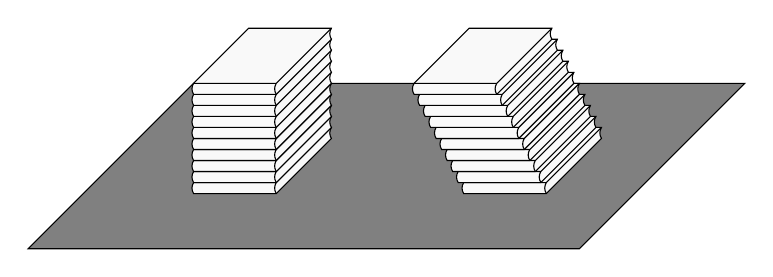
\begin{tikzpicture}[>=latex,scale=0.7,inner sep=1pt]
  \draw[fill=gray](-3,-1)--(7,-1)--(10,2)--(0,2)--cycle;
  \begin{scope}
  \foreach \y in {0,0.2,...,1.8}
    {
      \draw[fill=lightgray!10](0,\y)--(1.5,\y)--(2.5,1+\y)to[bend left](2.5,1.2+\y)--(1,1.2+\y)--(0,0.2+\y)to[bend right](0,\y)--cycle;
      \draw(1.5,\y)to[bend left](1.5,0.2+\y)--(2.5,1.2+\y)(1.5,0.2+\y)--(0,0.2+\y);
    }
  \end{scope}
  \begin{scope}[xshift=5cm]
  \foreach \y[count=\i] in {0,0.2,...,1.8}
    {
      \draw[fill=lightgray!10](-0.1*\i,\y)--(1.5-0.1*\i,\y)--(2.5-0.1*\i,1+\y)to[bend left](2.5-0.1*\i,1.2+\y)--(1-0.1*\i,1.2+\y)--(-0.1*\i,0.2+\y)to[bend right](-0.1*\i,\y)--cycle;
      \draw(1.5-0.1*\i,\y)to[bend left](1.5-0.1*\i,0.2+\y)--(2.5-0.1*\i,1.2+\y)(1.5-0.1*\i,0.2+\y)--(-0.1*\i,0.2+\y);
    }
  \end{scope}
\end{tikzpicture}
\end{document}